%%%%%%%%%%%%%%%%%%%%%%%%%%%%%%%%%%%%%%%%%%%%%%%%%%%%%%%%%%%%%%%%%%%%%%%%%%%%%%%%
% Inicializálás                                                                %
%%%%%%%%%%%%%%%%%%%%%%%%%%%%%%%%%%%%%%%%%%%%%%%%%%%%%%%%%%%%%%%%%%%%%%%%%%%%%%%%

%%%%%%%%%%%%%%%%%%%%%%%%%%%%%%%%%%%%%%%%%%%%%%%%%%%%%%%%%%%%%%%%%%%%%%%%%%%%%%%%
% Papírméret, betűméret, margó, magyar karakterek                              %
%%%%%%%%%%%%%%%%%%%%%%%%%%%%%%%%%%%%%%%%%%%%%%%%%%%%%%%%%%%%%%%%%%%%%%%%%%%%%%%%

\documentclass[a4paper,12pt]{article}
\special{papersize=210mm,297mm}

\usepackage{anysize}
\marginsize{2.5cm}{2.5cm}{2.5cm}{2.5cm}

\usepackage[utf8]{inputenc}
\usepackage[magyar]{babel}

%%%%%%%%%%%%%%%%%%%%%%%%%%%%%%%%%%%%%%%%%%%%%%%%%%%%%%%%%%%%%%%%%%%%%%%%%%%%%%%%
% Fedlap inicializálása                                                        %
%%%%%%%%%%%%%%%%%%%%%%%%%%%%%%%%%%%%%%%%%%%%%%%%%%%%%%%%%%%%%%%%%%%%%%%%%%%%%%%%

\usepackage{fedlap}

\csapat{unexpected\_exceptions}{59}
\konzulens{Ferencz Endre}

\taga{Biró Loránd}{NCZAGL}{lol.kylerrr@gmail.com}
\tagb{Kanyó Tibor}{NXWUKE}{kanyo.tibi@gmail.com}
\tagc{Magyar Dániel}{SUFFGT}{samuraidanm@gmail.com}
\tagd{Tarjáni Tamás}{S499KV}{tarjanitomi@gmail.com}
\tage{Vajsz Kornél}{VUYNAW}{roncsipar@gmail.com}

%%%%%%%%%%%%%%%%%%%%%%%%%%%%%%%%%%%%%%%%%%%%%%%%%%%%%%%%%%%%%%%%%%%%%%%%%%%%%%%%
% Fejléc és lábléc                                                             %
%%%%%%%%%%%%%%%%%%%%%%%%%%%%%%%%%%%%%%%%%%%%%%%%%%%%%%%%%%%%%%%%%%%%%%%%%%%%%%%%

\usepackage{fancyhdr}

\setlength{\headheight}{1.4em}
\setlength{\headsep}{2em}

\fancyhf{}
\fancyhead[OL] { \leftmark{} }
\fancyhead[OR] { \tmpcsapat }
\fancyfoot[OC] { \thepage }
\fancyfoot[OR] { \tmpdatum }

\pagestyle{fancy}

%%%%%%%%%%%%%%%%%%%%%%%%%%%%%%%%%%%%%%%%%%%%%%%%%%%%%%%%%%%%%%%%%%%%%%%%%%%%%%%%
% Napló                                                                        %
%%%%%%%%%%%%%%%%%%%%%%%%%%%%%%%%%%%%%%%%%%%%%%%%%%%%%%%%%%%%%%%%%%%%%%%%%%%%%%%%

\usepackage{longtable}

\newenvironment{journal}
{
	\hbadness 10000
	\begin{longtable}{|p{60pt}|l|l|p{216pt}|}
	\hline
	\textbf{Kezdet} & \textbf{Időtartam} & \textbf{Résztvevők} & \textbf{Leírás} \\
	\hline
	\endfirsthead
	\hline
	\textbf{Kezdet} & \textbf{Időtartam} & \textbf{Résztvevők} & \textbf{Leírás} \\
	\hline
	\endhead
}
{
	\end{longtable}
}

\newcommand{\journalentry}[4]
{
	{#1} & {#2} óra & \parbox{50pt}{#3} & {#4} \\
	\hline
}

%%%%%%%%%%%%%%%%%%%%%%%%%%%%%%%%%%%%%%%%%%%%%%%%%%%%%%%%%%%%%%%%%%%%%%%%%%%%%%%%
% UseCase leírás                                                               %
%%%%%%%%%%%%%%%%%%%%%%%%%%%%%%%%%%%%%%%%%%%%%%%%%%%%%%%%%%%%%%%%%%%%%%%%%%%%%%%%

\newenvironment{usecase}
{
	\hbadness 10000
	\begin{longtable}[l]{|p{100pt}|p{328pt}|}
	\hline
	\endfirsthead
	\hline
	\endhead
}
{
	\hline
	\end{longtable}
}

\newcommand{\usecaseentry}[2]
{
	\hline
	\textbf{#1} & {#2}\\
}

%%%%%%%%%%%%%%%%%%%%%%%%%%%%%%%%%%%%%%%%%%%%%%%%%%%%%%%%%%%%%%%%%%%%%%%%%%%%%%%%
% FileList leírás                                                               %
%%%%%%%%%%%%%%%%%%%%%%%%%%%%%%%%%%%%%%%%%%%%%%%%%%%%%%%%%%%%%%%%%%%%%%%%%%%%%%%%

\newenvironment{filelist}
{
	\hbadness 10000

	\begin{longtable}{|p{145pt}|p{35pt}|p{63pt}|p{163pt}|}
	\hline
	\textbf{Fájl neve} & \textbf{Méret} & \textbf{Keletkezés ideje} & \textbf{Tartalom} \\
	\hline
	\endfirsthead
	\hline
	\textbf{Fájl neve} & \textbf{Méret} & \textbf{Keletkezés ideje} & \textbf{Tartalom} \\
	\hline
	\endhead
}
{
	\end{longtable}
}

\newcommand{\filelistentry}[4]
{
	{#1} & {#2} b & {#3} & {#4} \\
	\hline
}
%%%%%%%%%%%%%%%%%%%%%%%%%%%%%%%%%%%%%%%%%%%%%%%%%%%%%%%%%%%%%%%%%%%%%%%%%%%%%%%%
% Egyebek                                                                      %
%%%%%%%%%%%%%%%%%%%%%%%%%%%%%%%%%%%%%%%%%%%%%%%%%%%%%%%%%%%%%%%%%%%%%%%%%%%%%%%%

\usepackage{graphicx}		% Kepek beillesztesehez
\usepackage{epstopdf}		% EPS fajlok felismeresehez
\graphicspath{{Images/}}	% Az Images mappaban keresse a kepeket

\anyag{11. Grafikus felület specifikációja}
\datum{2012. április 22.}
\setcounter{section}{10}

%%%%%%%%%%%%%%%%%%%%%%%%%%%%%%%%%%%%%%%%%%%%%%%%%%%%%%%%%%%%%%%%%%%%%%%%%%%%%%%%
% Dokumentum                                                                   %
%%%%%%%%%%%%%%%%%%%%%%%%%%%%%%%%%%%%%%%%%%%%%%%%%%%%%%%%%%%%%%%%%%%%%%%%%%%%%%%%

\begin{document}

\fedlap

\section{Grafikus felület specifikációja}

\subsection{A grafikus interfész}

\subsection{A grafikus felület architektúrája}

\subsubsection{A felület működési elve}

Az eddig elkészült rendszer a játékszabályokat ismeri és magának a játéknak a szimulálására képes, de az olyan magas szintű funkciók mint a megjelenítés, a menürendszer vagy az inputok figyelése nem ismert a számára. Ezek a logikák a most tervezett osztályokban valósulnak meg. Az eddig elkészült \emph{gameLogic} package-et csak a \emph{GameScene} használja, amikor betölti az aktuális \emph{Level} objektumot minden \emph{GameObject}-hez létrehoz egy ahhoz tartozó \emph{IDrawableGameComponent} objektumot ami annak a megjelenítéséért felelős. (A 6. osztálydiagram ezeket a kapcsolatokat mutatja.) A kiírásban szereplő definíciók alapján az alapelv se nem pull, se nem push, mert az \emph{IDrawableGameComponent} objektumok csak a \emph{GameObject} osztályok aktuális állapotát rajzolják ki és semmilyen esemény nincs értelmezve a játéklogikában amiről "értesülne" a megjelenítés. De amennyiben muszáj lenne választani akkor nyilván pull lenne, mert a játéklogikát megvalósító osztályok semmilyen formában nem tudnak a megjelenítési rétegről. Ez az architektúra a játéklogika könnyű tesztelhetőségét tette lehetővé.

\subsubsection{A felület osztály-struktúrája}

\graphicspath{{PdfImages/}}
\begin{center}
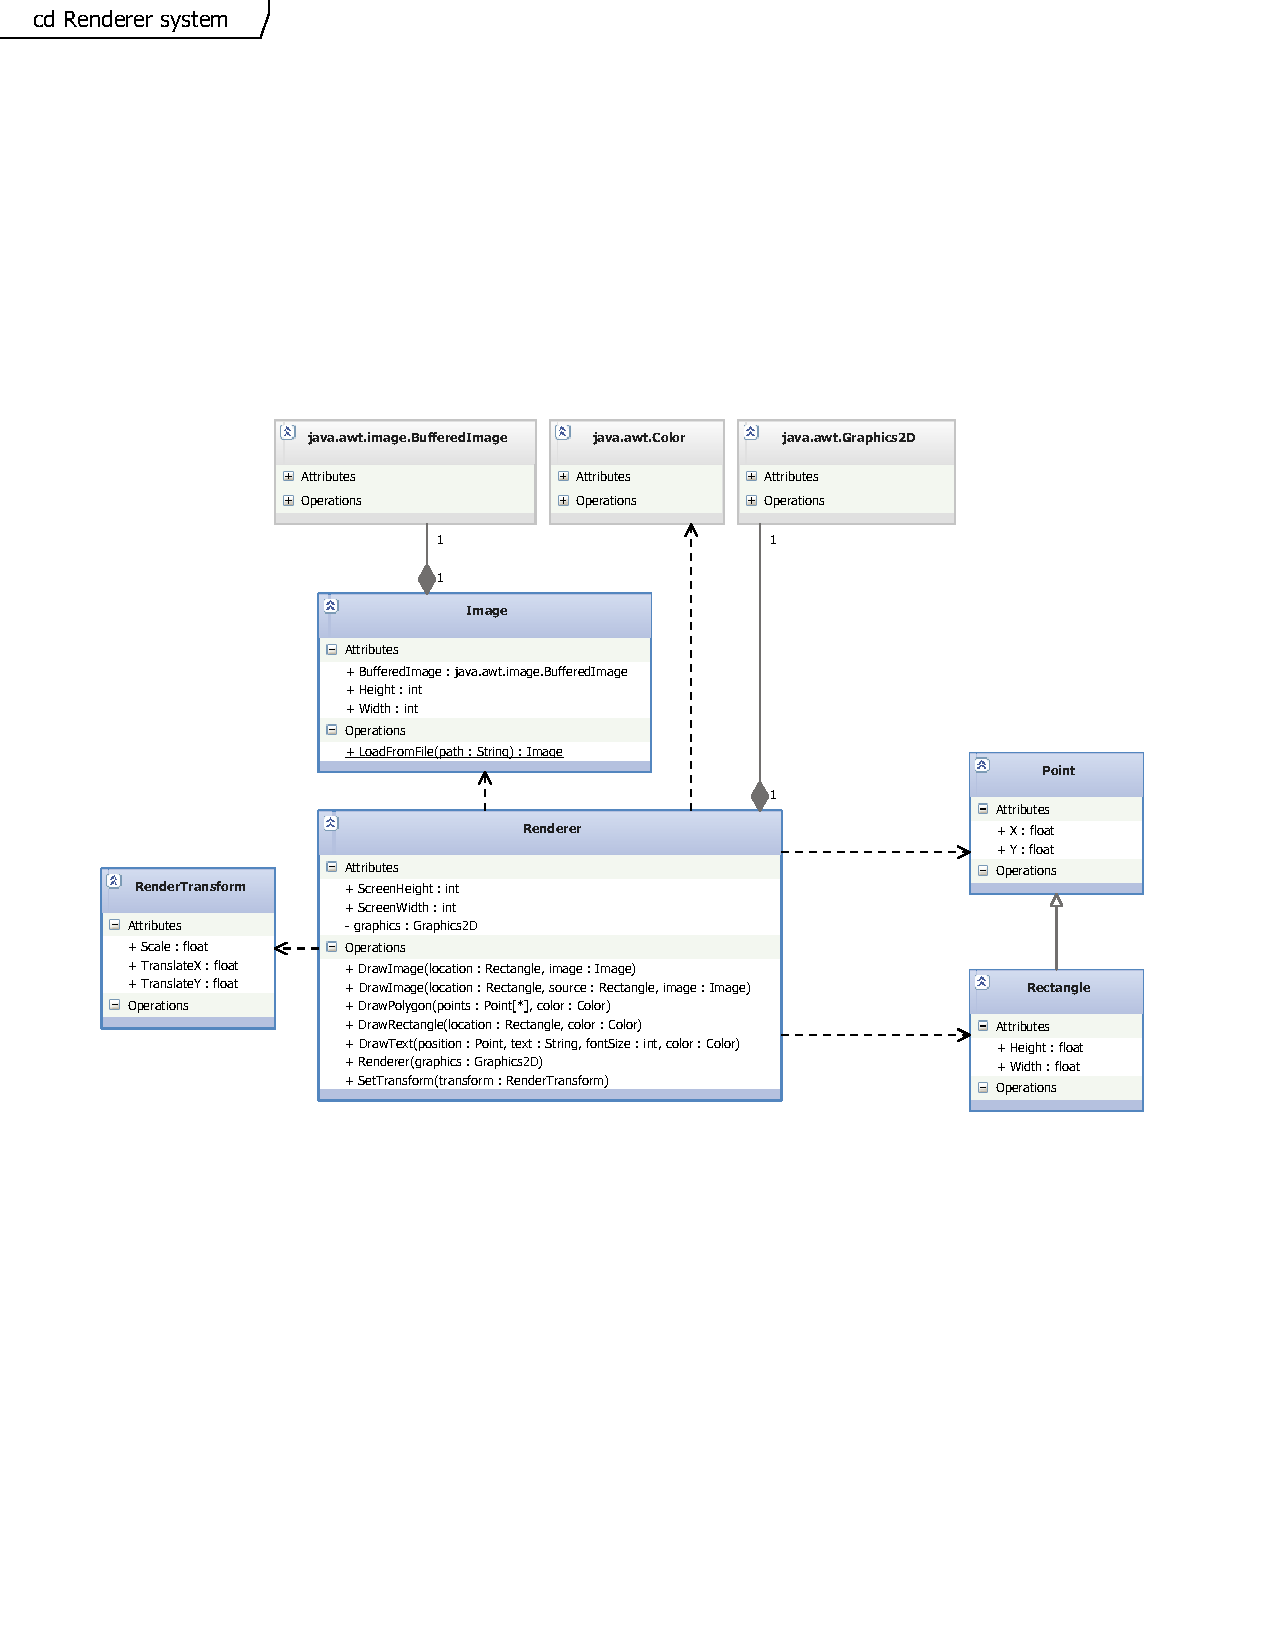
\includegraphics[scale=0.7]{Renderer.pdf}
\newpage
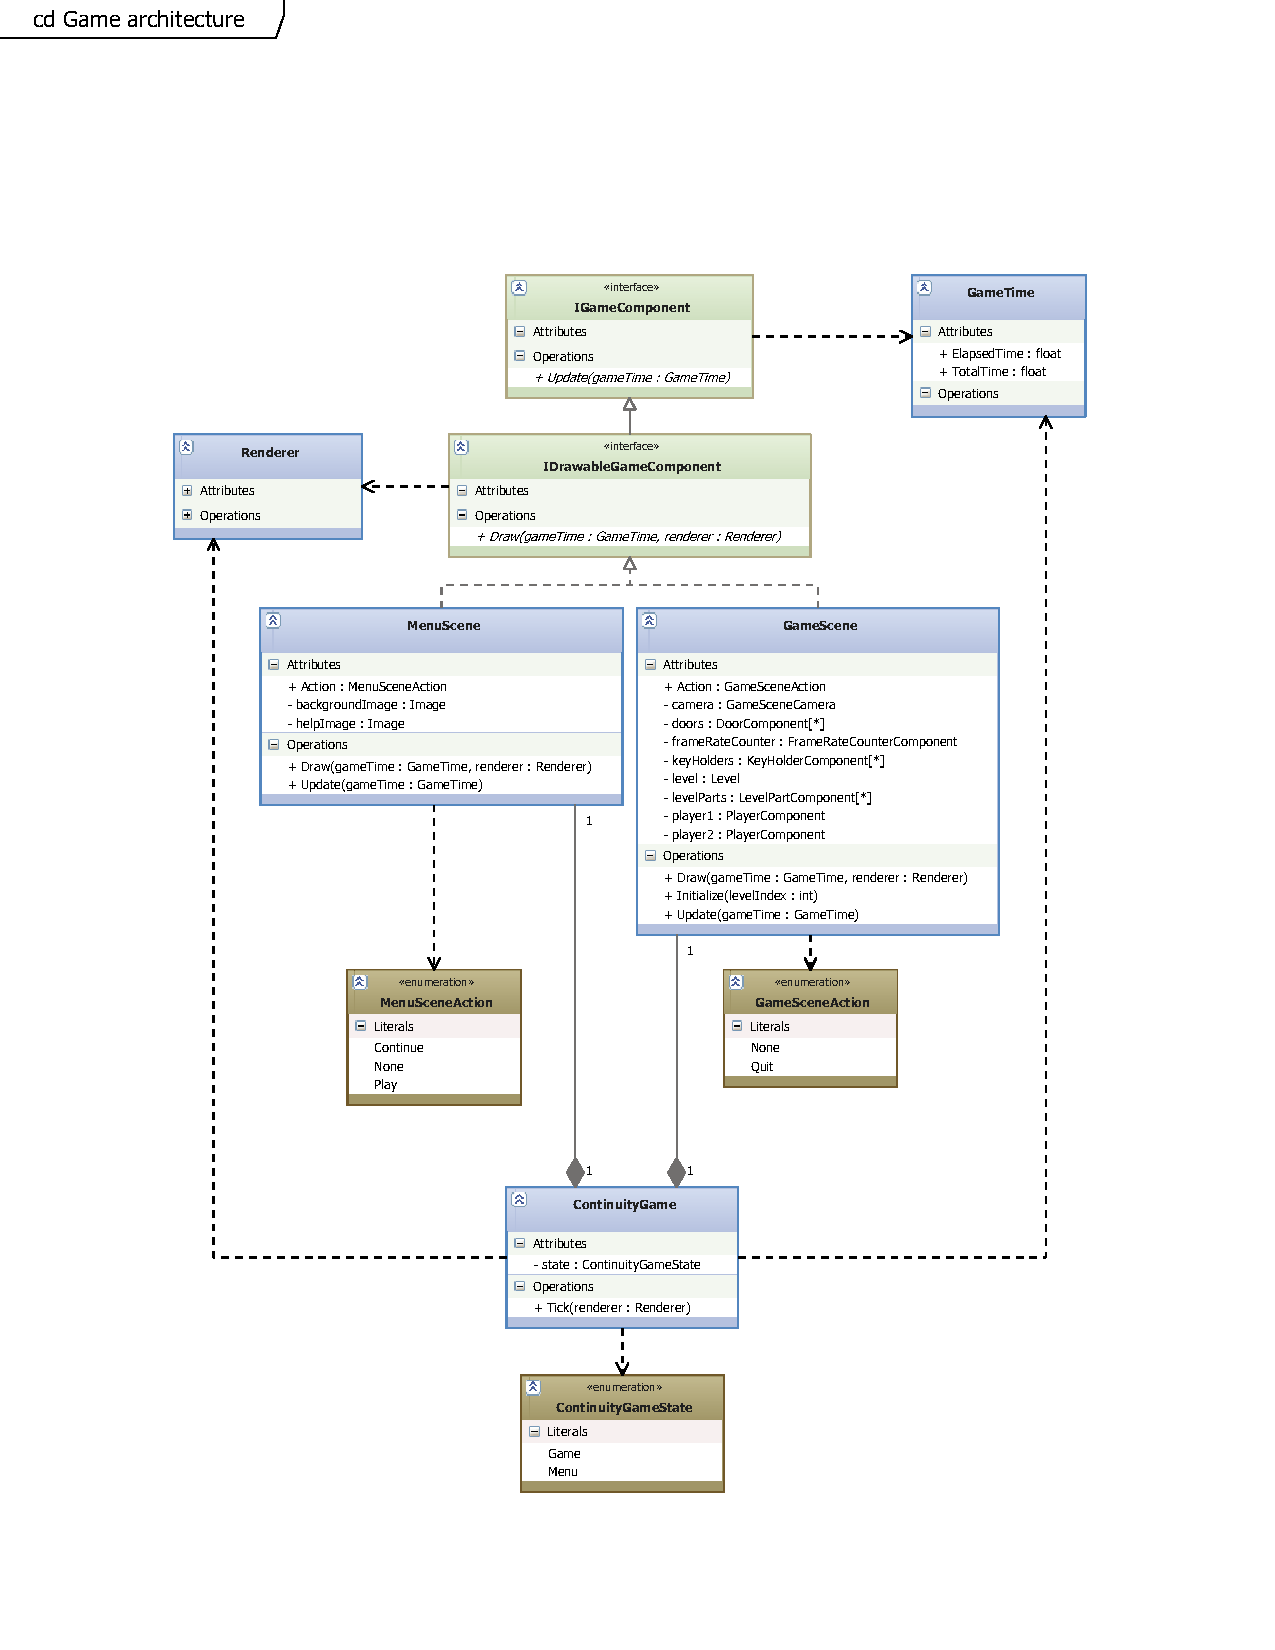
\includegraphics[scale=0.7]{GameArchitecture.pdf}
\newpage
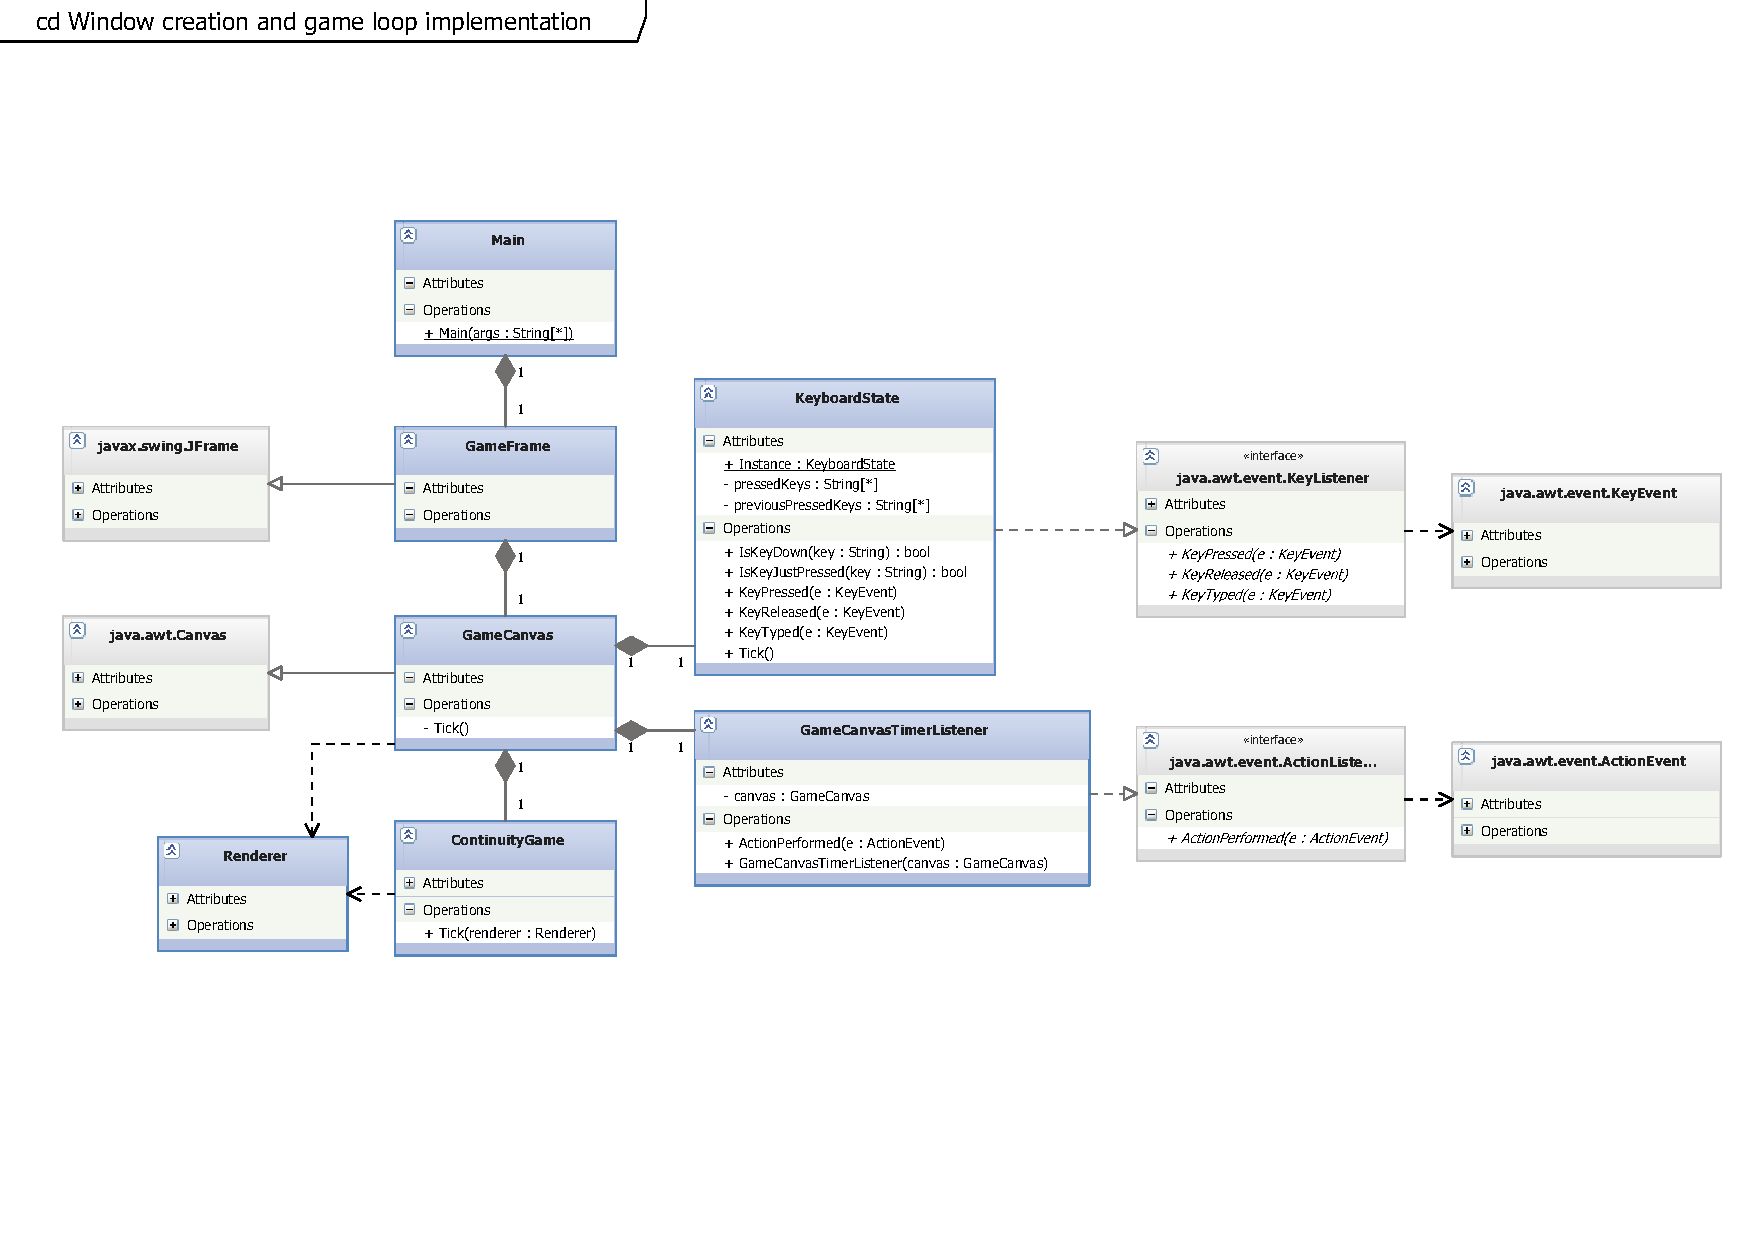
\includegraphics[scale=0.7,angle=90]{Main.pdf}
\newpage
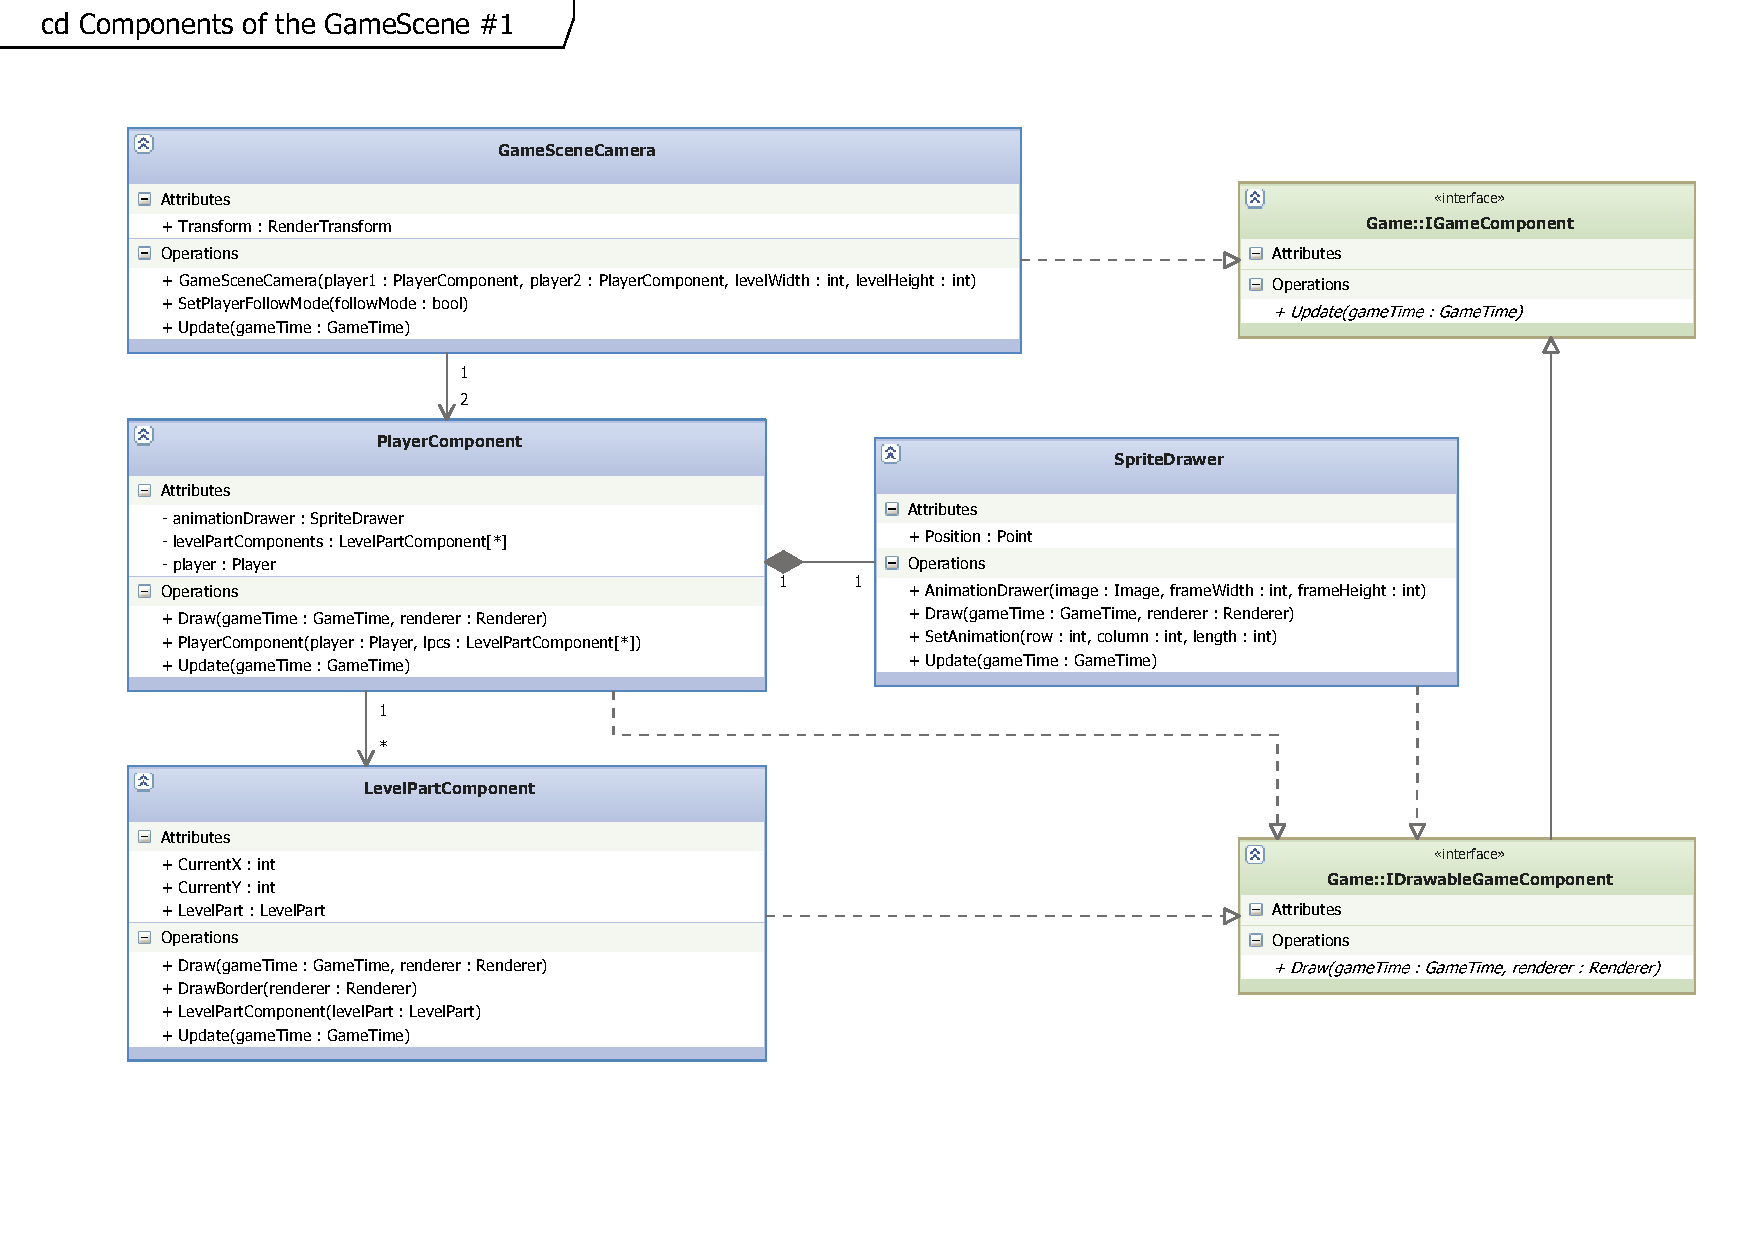
\includegraphics[scale=0.7,angle=90]{GameSceneComponents.pdf}
\newpage
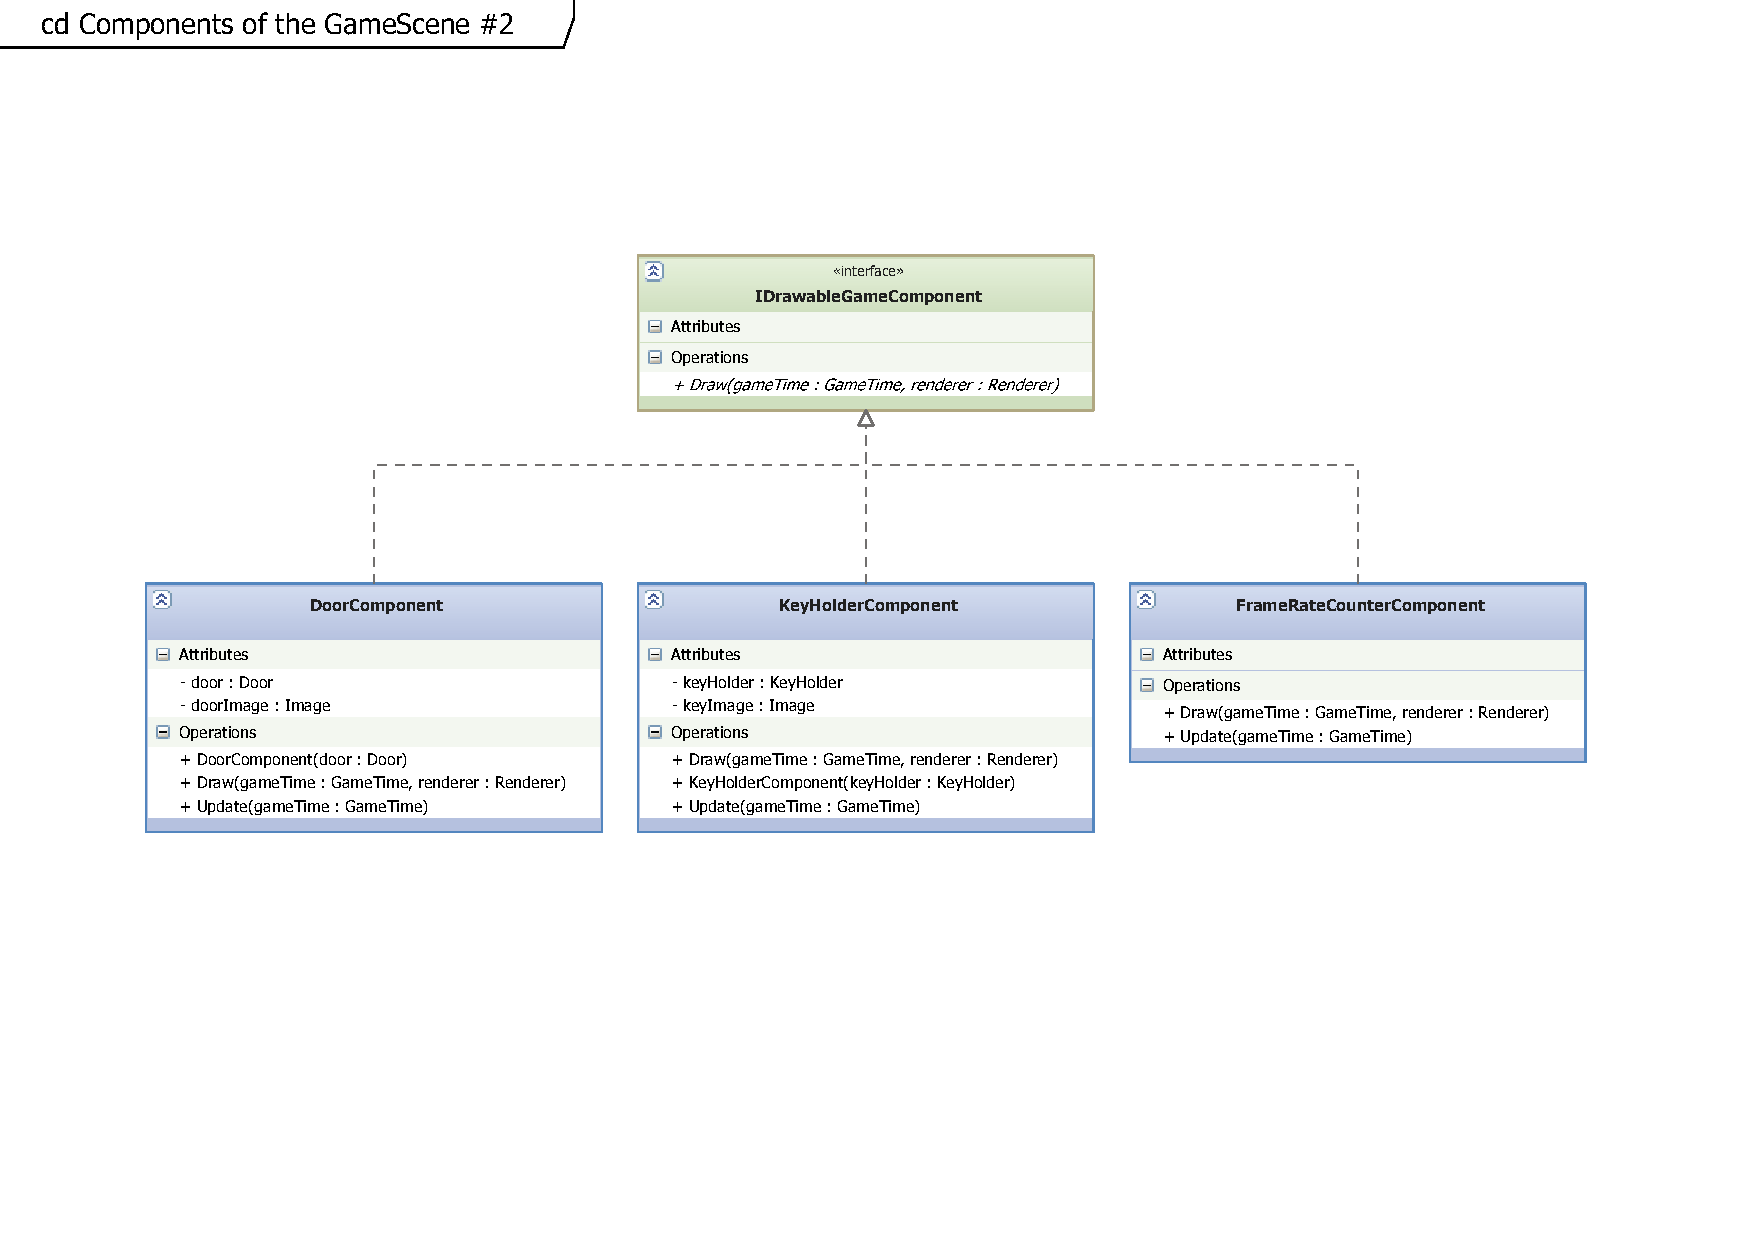
\includegraphics[scale=0.7,angle=90]{GameSceneComponents2.pdf}
\newpage
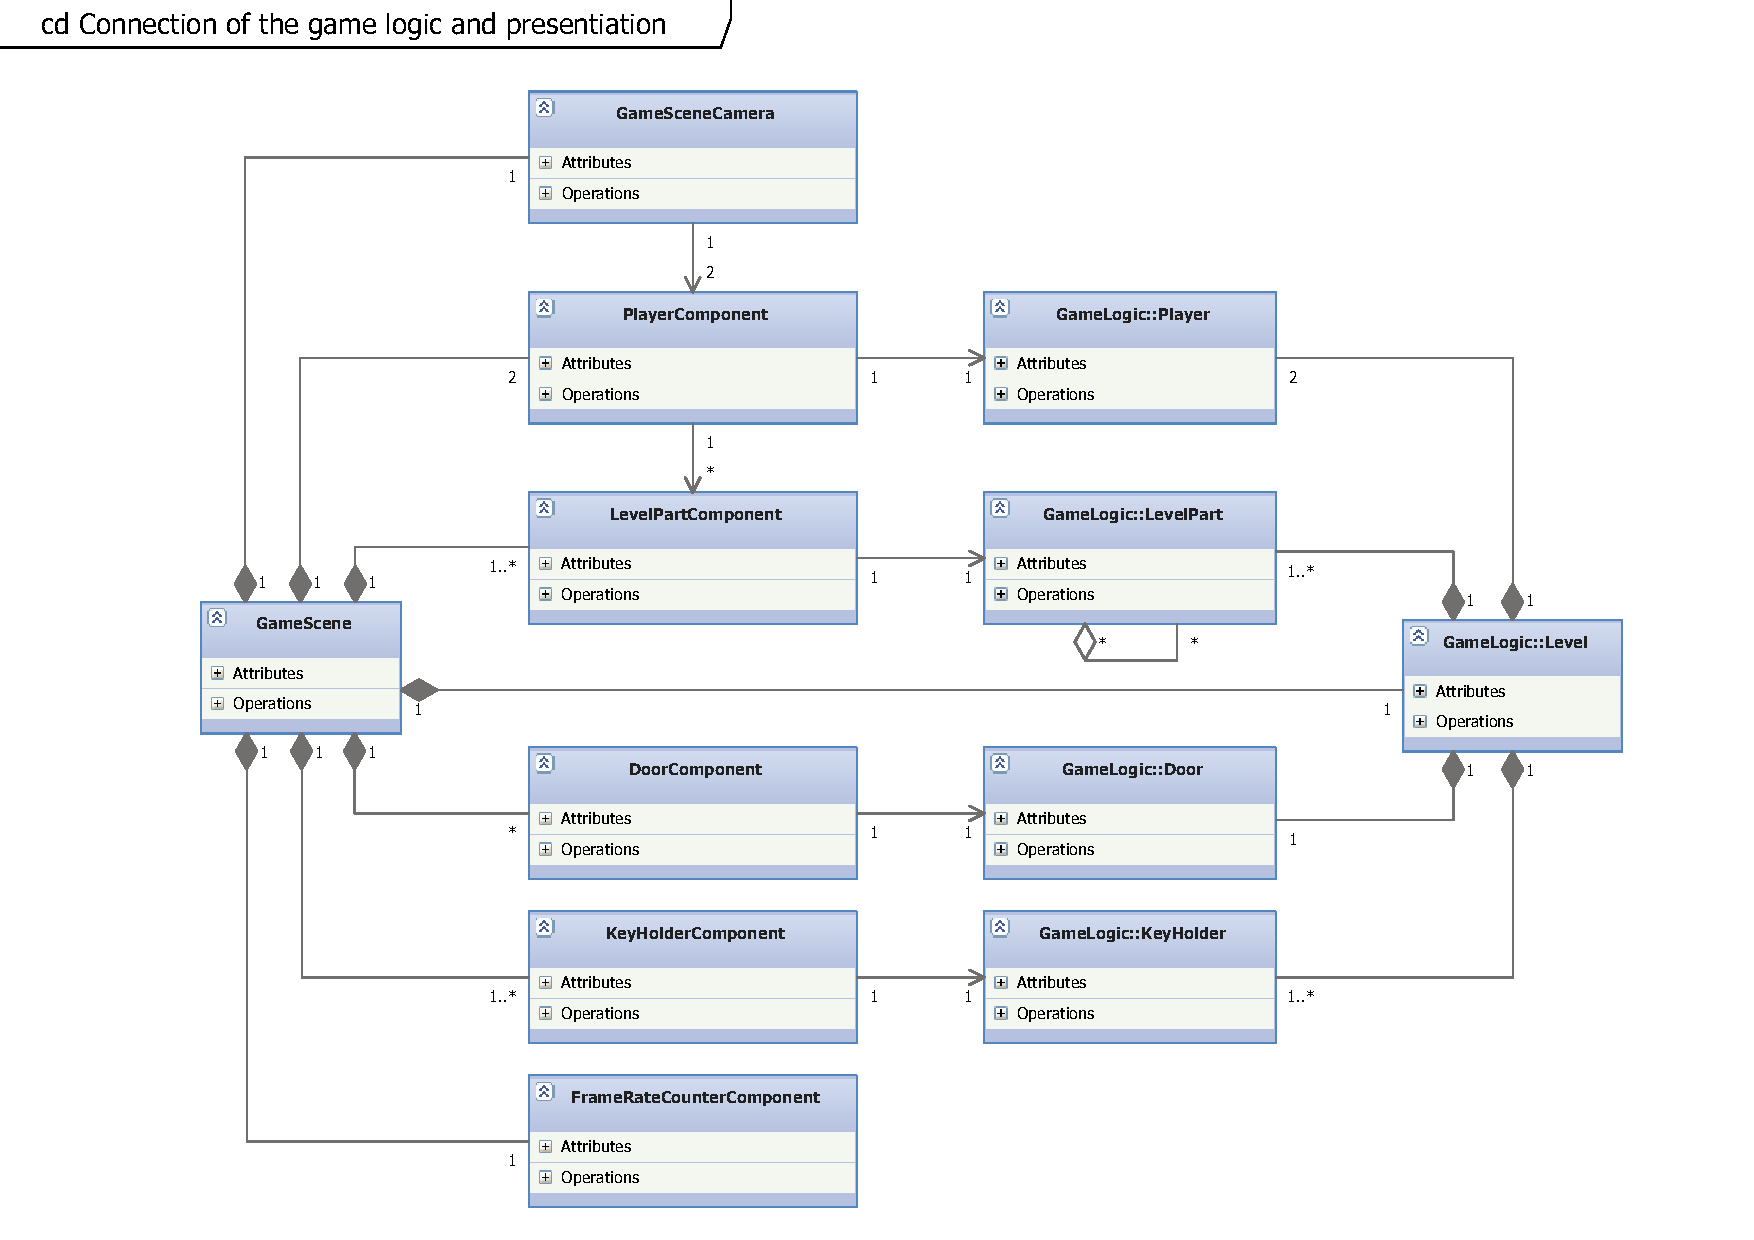
\includegraphics[scale=0.7,angle=90]{GameLogicPresentationConnection.pdf}
\newpage
\end{center}

\subsection{A grafikus objektumok felsorolása}
Amelyik osztály leírásánál nem szerepel az Ősosztályok vagy az Interfészek pont, annak az osztálynak értelemszerűen nincs őse vagy nem valósít meg interfészt. Az összes, a leírásban szereplő attribútum és metódus publikus.

\subsubsection{Point}
	\begin{description}
		\item[Felelősség] \hfill \\
		Egy pontnak felel meg a koordináta-síkon.
		
		\item[Attribútumok]\hfill \\
		\textbf{\emph{float X}}: A pont x koordinátája.
		
		\textbf{\emph{float Y}}: A pont y koordinátája.		
				
		\item[Metódusok]\hfill \\
		-

	\end{description}
	
\subsubsection{Rectangle}
	\begin{description}
		\item[Felelősség] \hfill \\
		Egy téglalapot leíró osztály.
		
		\item[Ősosztályok] \hfill \\
		A {\itshape Point}	osztályból származik.		
		
		\item[Attribútumok]\hfill \\
		\textbf{\emph{float Height}}: A téglalap magassága.
		
		\textbf{\emph{float Width}}: A téglalap szélessége.		
				
		\item[Metódusok]\hfill \\
		-

	\end{description}
	
\subsubsection{Image}
	\begin{description}
		\item[Felelősség] \hfill \\
		Egy képet leíró osztály. Képes fájlból betölteni a képet, és bizonyos méretűre formázni.
		
		\item[Attribútumok]\hfill \\
		
		\textbf{\emph{BufferedImage BufferedImage}}: Egy java.awt.image.BufferedImage típusú változó, amiben a betöltött képet tároljuk.
		
		\textbf{\emph{int Height}}: A betöltött kép magassága.	
		
		\textbf{\emph{int Width}}: A betöltött kép szélessége.	
				
		\item[Metódusok]\hfill \\
		\textbf{\emph{LoadFromFile(String)}}: A paraméterként kapott elérési útról betölt egy képet.

	\end{description}
	
\subsubsection{RenderTransform}
	\begin{description}
		\item[Felelősség] \hfill \\
		Transzformációt leíró osztály.
		
		\item[Attribútumok]\hfill \\
		\textbf{\emph{float Scale}}: A transzformáció aránya, vagyis hogy hányszorosára növeljük a transzformálandó objektumot (képet, stb.).
		
		\textbf{\emph{float TranslateX}}: X koordináta szerinti transzformáció (az x tengely mentén mennyire nyomjuk össze vagy nyújtjuk a transzformált objektumot).	
		
		\textbf{\emph{float TranslateY}}: Y koordináta szerinti transzformáció.	
				
		\item[Metódusok]\hfill \\
		-

	\end{description}

\subsubsection{Renderer}
	\begin{description}
		\item[Felelősség] \hfill \\
		Lényegében ez az osztály felel a grafikus megjelenítésért, ez végzi a kirajzolásokat és a {\itshape RenderTransform} által leírt transzformációkat is.
		
		\item[Attribútumok]\hfill \\
		\textbf{\emph{int ScreenHeight}}: A játékot megjelenítő ablak magassága.
		
		\textbf{\emph{int ScreenWidth}}: A játékot megjelenítő ablak szélessége.		
				
		\item[Metódusok]\hfill \\
		\textbf{\emph{DrawImage(Rectangle, Image)}}: A paraméterként kapott képet kirajzolja a megadott téglalap által meghatározott helyre.
		
		\textbf{\emph{DrawImage(Rectangle, Rectangle, Image)}}: Az előző metódustól abban különbözik, hogy a második Rectangle paraméter segítségével kijelölhetjük a képből a megjelenítendő területet.
		
		\textbf{\emph{DrawPolygon(Point*[], Color)}}: Egy poligont rajzol fel, aminek a csúcsait egy, a pontokra mutató pointereket tartalmazó tömbben kapja meg. A poligon színét a {\itshape Color} típusú paraméter határozza meg.
		
		\textbf{\emph{DrawRectangle(Rectangle, Color)}}: Kirajzolja a paraméterként kapott téglalapot a megadott színnel.
		
		\textbf{\emph{DrawText(Point, String, int, Color)}}: Adott szöveget rajzol ki a kapott ponttól kezdődően az int paraméter által meghatározott betűmérettel és a megadott színnel.
		
		\textbf{\emph{SetTransform(RenderTransform)}}: Beállíthatjuk a használt kameratranszformációt.
						
	\end{description}
	
	
\subsubsection{IGameComponent}
	\begin{description}
		\item[Felelősség] \hfill \\
		Minden, a játékban résztvevő objektumnak változhat időben az állapota, azok számára egy interfész. Azoknak kell rendelkezni egy olyan metódussal, amivel lehet frissíteni az állapotokat az eltelt idő alapján.

		\item[Metódusok]\hfill \\
		\textbf{\emph{Update(GameTime)}}: Az interfészt megvalósító objektum szimulációs metódusának deklarálása.
	\end{description}
	
\subsubsection{GameTime}
	\begin{description}
		\item[Felelősség] \hfill \\
		A mozgások szimulálásánál a szükséges eltelt idők meghatározásához használt struktúra.
		
		\item[Attribútumok]\hfill \\
		\textbf{\emph{float ElapsedTime}}: A struktúra példányosításakor az előző lekéréstől számított eltelt idő másodpercben.

		\textbf{\emph{float TotalTime}}: A struktúra példányosításakor a játék futásának ideje másodpercben.
	\end{description}
	
\subsubsection{IDrawableGameComponent}
	\begin{description}
		\item[Felelősség] \hfill \\
		A grafikus felületen megjeleníthető	objektumok számára egy interfész. Ebből vannak leszármaztatva, így a program futása közben tökéletes szétválaszthatók az egyszerű objektumoktól azok, amely a grafikus felületen is megjelenhetnek.

		\item[Ősosztályok] \hfill \\
		DrawableGameComponent

		\item[Metódusok]\hfill \\
		\textbf{\emph{Draw(GameTime,Renderer)}}: Adott időre vonatkozó rajzolómetódus deklarálása. 
	\end{description}

\subsubsection{MenuScene}
	\begin{description}
		\item[Felelősség] \hfill \\
		A menü működéséért, megjelenítésért felelős objektum.

		\item[Interfészek]\hfill \\
		IDrawableGameComponent

		\item[Attribútumok]\hfill \\
		\textbf{\emph{Action MenuSceneAction}}: Éppen aktuálisan beállított esemény, amelyet a felhasználó váltott ki a menüben. Például új játékot szeretne indítani.

		\item[Metódusok]\hfill \\
		\textbf{\emph{Draw(GameTime,Renderer)}}: A menüben lévő kirajzolható objektumokra sorban meghívja a saját rajzolási metódusokat.

		\textbf{\emph{Update(GameTime)}}: Az inputok alapján eldönteni, hogy milyen értéke legyen a MenuSceneAction attribútumnak.
	\end{description}


\subsubsection{MenuSceneAction}
	\begin{description}
		\item[Felelősség] \hfill \\
		A felhasználó a menüben különböző eseményeket tud generálni, például új játékot indíthat. Ezen osztály a menüben kiadható eseményeket sorolja fel. Lehetséges értékek: None, Play, Continue.
	\end{description}
	
\subsubsection{GameScene}
	\begin{description}
		\item[Felelősség] \hfill \\
		Egy-egy pálya működéséért, megjelenítésért felelős objektum.
		\item[Interfészek]\hfill \\
		IDrawableGameComponent
		\item[Attribútumok]\hfill \\
		\textbf{\emph{Action GameSceneAction}}: Éppen aktuálisan beállított esemény, amelyet a felhasználó váltott ki adott pályához kapcsolódóan.

		\item[Metódusok]\hfill \\
		\textbf{\emph{Draw(GameTime,Renderer)}}: A pályán lévő kirajzolható objektumokra sorban meghívja a saját rajzolási metódusokat.

		\textbf{\emph{Update(GameTime)}}: A pályán lévő objektumokra leszimulálja a mozgást a megadott időtartamra.
	\end{description}
	
\subsubsection{GameSceneAction}
	\begin{description}
		\item[Felelősség] \hfill \\
		A felhasználó eseményeket generálhat gombnyomásra, például kiléphet a játékból. Ezen osztály a pályán kiadható eseményeket sorolja fel. Lehetséges értékek: None, Quit.
	\end{description}
	
\subsubsection{ContinuityGame}
	\begin{description}
		\item[Felelősség] \hfill \\
		A különböző jelenetek, scene-k közötti átváltásokat kezeli. Ezen osztály dönti el, hogy melyik jelenetet kell betölteni.
		\item[Metódusok]\hfill \\
		\textbf{\emph{Tick(Renderer)}}: Meghívja az aktuális scene Update és Draw metódusát, majd ezt követően megvizsgálja, hogy kell-e váltani másik scene-re.
	\end{description}
	
	
	
\subsubsection{GameSceneCamera}
	\begin{description}
		\item[Felelősség] \hfill \\
		A teljes játéktérből a megfelelő síkrészt láttatja.
		\item[Interfészek] \hfill \\
		IGameComponent
		\item[Attribútumok] \hfill \\
		\textbf{\emph{RenderTransform Transform}}: A kamera transzformáció-beállításait tárolja.

		\item[Metódusok] \hfill \\
		\textbf{\emph{Update(GameTime)}}: Beállítja a transzformációját a kamerának.

		\textbf{\emph{SetPlayerFollowMode(Boolean)}}: Megadjuk, hogy a játékosokat követő vagy a tili-toli módban vagyunk.
		
		\textbf{\emph{GameSceneCamera(PlayerComponent player1, PlayerComponent player2, int levelWidth, int levelHeight}}: Megadjuk, hogy mely játékos modelleket figyeljen a kamera, illetve a pálya méretét is átadjuk neki.
	\end{description}

\subsubsection{PlayerComponent}
	\begin{description}
		\item[Felelősség] \hfill \\
		A játékos megjelenítését vezérlő osztály.
		\item[Interfészek] \hfill \\
		IDrawableGameComponent
		\item[Attribútumok] \hfill \\
		\textbf{\emph{SpriteDrawer spriteDrawer}}: A játékos animált mozgásának megjelenítését valósítja meg.

		\item[Metódusok] \hfill \\
		\textbf{\emph{Draw(GameTime,Renderer)}}: Továbbhívja a spriteDrawer objektum Draw metódusára, amely aztán kirajzolja a megfelelő állapotát a játékosnak.

		\textbf{\emph{Update(GameTime)}}: Frissíti a játékos pozícióját a spriteDrawer számára, majd meghívja annak az Update metódusát.

		\textbf{\emph{PlayerComponent(Player, LevelPartComponent[])}}: Megadjuk, hogy melyik játékos objektumra vonatkozik a megjelenítés, és átadjuk a pályaelemeket listáját.
		
	\end{description}
	

\subsubsection{SpriteDrawer}
	\begin{description}
		\item[Felelősség] \hfill \\
		A játékosok animált mozgását megvalósító osztály.
		\item[Interfészek] \hfill \\
		IDrawableGameComponent
		\item[Attribútumok] \hfill \\
		\textbf{\emph{Point Position}}: Hova kell rajzolni a kívánt képet.

		\item[Metódusok] \hfill \\
		\textbf{\emph{SpriteDrawer(Image image,int frameWidth, int frameHeight)}}: Megadjuk azt a képet, amelyen szerepelnek a kívánt képkockák az animáláshoz, illetve egy képkocka méretét.

		\textbf{\emph{SetAnimation(int row, int column, int length}}: Beállítja, hogy az adott képsorozatból melyik képkockától kezdve mennyi képkockát kell az adott mozgásnál ismételni.

		\textbf{\emph{Draw(GameTime,Renderer)}}: Kirajzolja a megfelelő képkockát/képkockákat a sorozatból

		\textbf{\emph{Update(GameTime)}}: Meghatározza, hogy mely képkockákat kell kirajzolni.
		
	\end{description}
	
\subsubsection{LevelPartComponent}
	\begin{description}
		\item[Felelősség] \hfill \\
		Egy adott pályaelem megjelenítésért felelős osztály.
		\item[Interfészek] \hfill \\
		IDrawableGameComponent

		\item[Attribútumok] \hfill \\
		\textbf{\emph{int CurrentX}}: A pályaelem x koordinátája.

		\textbf{\emph{int CurrentY}}: A pályaelem y koordinátája.

		\textbf{\emph{LevelPart LevelPart}}: A megadott objektum, amely alapján történik a kirajzolás.
		
		\item[Metódusok] \hfill \\
		\textbf{\emph{LevelPartComponent(LevelPart)}}: Konstruktorban megadjuk a pályaelem objektumát.

		\textbf{\emph{Draw(GameTime,Renderer)}}: Kirajzolja a pályaelemet.

		\textbf{\emph{DrawBorder(Renderer)}}: A pályaelem külső keretét rajzolja ki.

		\textbf{\emph{Update(GameTime)}}: Frissíti a pályaelemek pozícióját.
	\end{description}
	
\subsubsection{DoorComponent}
	\begin{description}
		\item[Felelősség] \hfill \\
		Az ajtót megjelenítő osztály.
		\item[Interfészek] \hfill \\
		IDrawableGameComponent

		\item[Metódusok] \hfill \\
		\textbf{\emph{DoorComponent(Door)}}: Konstruktorba lehet megadni, hogy melyik ajtó objektumhoz tartozzon a kirajzoltatás.

		\textbf{\emph{Draw(GameTime,Renderer)}}: Kirajzolja az ajtót.

		\textbf{\emph{Update(GameTime)}}: Pusztán az interfész követeli meg a létét, semmit nem csinál.
	\end{description}
	
\subsubsection{KeyHolderComponent}
	\begin{description}
		\item[Felelősség] \hfill \\
		A kulcsot megjelenítő osztály.
		\item[Interfészek] \hfill \\
		IDrawableGameComponent

		\item[Metódusok] \hfill \\
		\textbf{\emph{KeyHolderComponent(KeyHolder)}}: Konstruktorba lehet megadni, hogy melyik kulcs objektumhoz tartozzon a kirajzoltatás.

		\textbf{\emph{Draw(GameTime,Renderer)}}: Kirajzolja a kulcsot.

		\textbf{\emph{Update(GameTime)}}: Pusztán az interfész követeli meg a létét, semmit nem csinál.
	\end{description}
	
\subsubsection{FrameRateCounterComponent}
	\begin{description}
		\item[Felelősség] \hfill \\
		Folyamatosan kiszámolja, hogy hány képkockát rajzolunk ki másodpercenként.
		\item[Interfészek] \hfill \\
		IDrawableGameComponent

		\item[Metódusok] \hfill \\
		\textbf{\emph{Draw(GameTime,Renderer)}}: Kirajzolja az aktuális értéket.

		\textbf{\emph{Update(GameTime)}}: Kiszámolja az értékét.
	\end{description}
	
\subsection{Kapcsolat az alkalmazói rendszerrel}

\subsection{Napló}

\begin{journal}
\journalentry{2012.04.04. 13:30}{2}{Biró, Kanyó, Magyar, Tarjáni, Vajsz}{Értekezlet, döntés a grafikus megjelenítés mikéntjéről, a feladatok kiosztása.}
\journalentry{2012.04.22. 14:00}{1}{Tarjáni}{Dokumentumsablon, osztályleírások elkészítése.}
\journalentry{2012.04.22. 16:00}{2}{Kanyó}{Osztályleírások bővítése, javítása.}

\end{journal}

\end{document}